\section[MODELO DE GESTÃO]{MODELO DE GESTÃO}
O software terá um modelo de gestão baseado no método \emph{SCRUM}, como definido em \ref{scrum_sec}.
O método não é adotado na plenitude, sendo adaptado segundo as limitações de recursos do projeto.

Nesta fase inicial, o processo conta com um desenvolvedor, que também assume o papel de \emph{scrum master}, e um \emph{product owner}. 
Devido ao tamanho reduzido da equipe e da localização distinta dos membros, não há \emph{daily scrum}, mas problemas de trabalho cotidianos são resolvidos por telefone, \emph{email} ou mensagens instantâneas. 

O princípio de \emph{time boxing} é mantido. Ficou definido que o \emph{sprint} consiste do prazo de duas semanas. Ao final do \emph{sprint} uma reunião em duas fases é realizada. A primeira fase consiste na revisão do \emph{sprint} anterior. Já a segunda fase é o planejamento do próximo \emph{sprint}.

Um \emph{backlog} de produto é mantido. Na reunião de final de \emph{sprint} é criado um \emph{backlog} de \emph{sprint}. 
Os itens de \emph{backlog} são mantidos na forma de estórias de usuários, conforme \ref{user_stories_sec}.
Na Figura \ref{scrum_projeto} é apresentada a visão geral do processo.

\begin{figure}[ht]
	\centering
	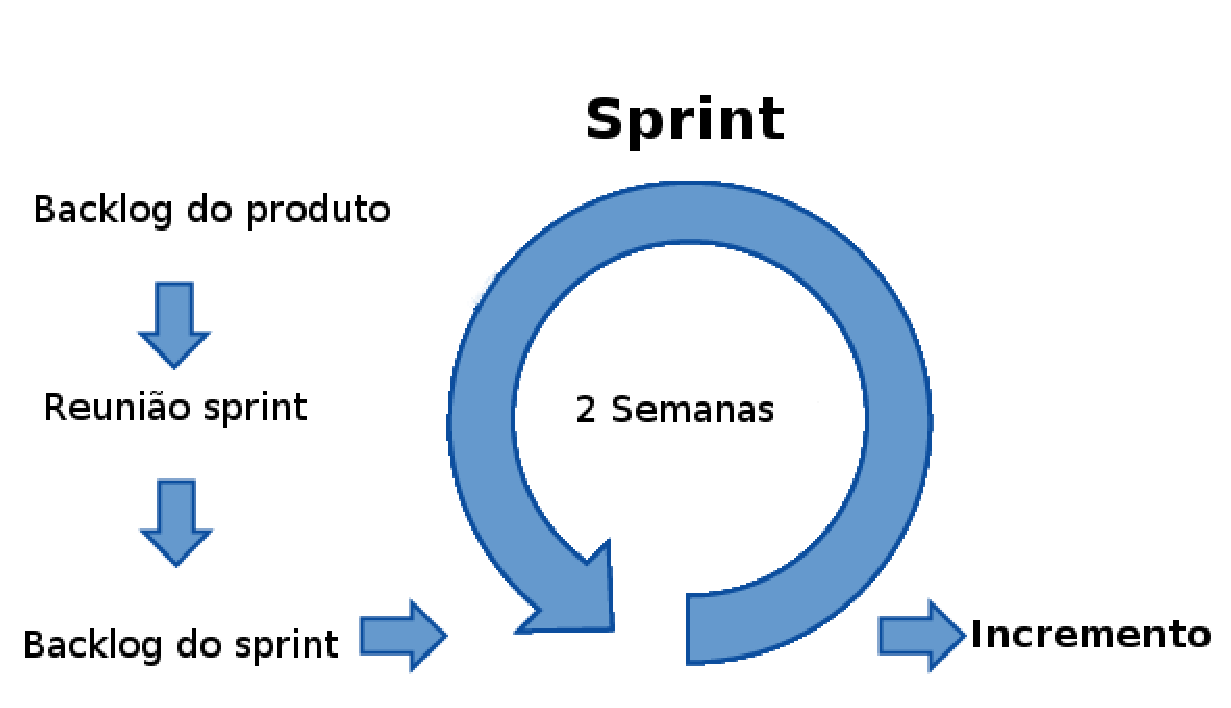
\includegraphics[width=15cm]{figuras/scrum_projeto.eps}
	\caption{Processo de desenvolvimento.}
	\label{scrum_projeto}
\end{figure}





